\chapter{TreeSwiftの設計と実装}
\label{experiment}

本章では、本研究の提案手法であるLEONの評価を行う。

\section{実装の概要}
\label{applicationperformance}

~\ref{solv:requirements}節で示した通り、機能要件は、1. インターネット上に分散された複数の拠点へのLayer 2ネットワークの拡張、
2. 宛先に応じた転送先の選択、3. 遅延の最も小さい経路でのイーサネットフレームの転送、4. 分散して動作すること、の4つである。機能要件に
ついて、LEONと~\ref{rw:pointtopoint}節と~\ref{rw:pointtomulti}節で挙げた既存研究が、どの程度満たしてるかを表~\ref{table:relatedworksandleon}
に示す。

\begin{table}[h]
	\begin{center}
		\caption{LEONと既存研究の比較}
		\begin{tabular}{|l|c|c|c|c|}
			\hline
			機能要件 & GRE/L2TP & VXLAN & N2N & LEON \\
			\hline
			\hline
			1. インターネット上の複数環境への拡張 & × & × & ◯ & ◯ \\
			\hline
			2. 宛先に応じた転送先の選択 & × & ◯ & ◯ & ◯ \\
			\hline
			3. 遅延の最も小さい経路での転送 & × & × & × & ◯ \\
			\hline
			4. 分散して動作する & × & ◯ & × & ◯ \\
			\hline
		\end{tabular}
		\label{table:relatedworksandleon}
	\end{center}
\end{table}

GREやL2TPなどといった一対一型のLayer 2ネットワーク拡張技術は、どの機能要件も満たしていない。
一方、VXLANとN2Nは一対多型のLayer 2ネットワーク拡張技術のため、両者共に機能要件の2は満たしている。しかし、両者共に遅延の最も小さい経路でイーサネット
フレームを機能を転送する機能がないため、機能要件の3を満たしていない。インターネット上に分散した複数の拠点にLayer 2ネットワークを拡張するLEONは、
トンネル終端点間の遅延を計測し、計測結果から遅延の最も小さい経路を計算することができる。そして、イーサネットフレームを転送する際に、遅延の最も
小さい経路で転送することができる。そのため、機能要件の1、2、3を満たす。また、N2NはSupernode
を必要とするため、機能要件の4を満たさない。VXLANとLEONは分散して動作するため、機能要件の4を満たす。
以上より、LEONは機能要件を全て満たしている。

LEONはインターネット上に分散した複数の拠点を用いて展開されたサービスのパフォーマンスを向上させることを目標としている。
これを実現するために、LEONはLayer 2ネットワークのイーサネットフレームを遅延の最も小さい経路で転送をする。これにより、
サービスを構成するコンポーネントの通信パフォーマンスが向上し、サービスのパフォーマンスが向上すると予想される。そこで
本研究では、LEONが与えるサービスのパフォーマンスへの影響を評価する。

しかし、一方でLEONは全てのトンネル終端点が、全てのトンネル終端点までの遅延計測や死活監視を行なっている。また、ブロードキャストフレーム
やコントロールメッセージを全てのトンネル終端点に転送する。そのため、トンネル終端点の台数が増加するとLEONに悪影響を与える
と予想される。そこで本研究では、トンネル終端点の増加がLEONに与える影響の評価も行う。

\section{構文解析}

本研究ではまず、LEONが遅延の最も小さい経路でイーサネットフレームを転送することによって、サービスのパフォーマンス
に与える影響を評価する。本評価を行うにあたり、インターネット上に分散された複数の拠点を用いて構築されたサービス
の例としてWIDE Cloudを用いる。

WIDE Cloudには、~\ref{wcclatency}項で説明したように、複数の拠点でサービスを構築
した場合、コンポーネントのパフォーマンスが低下するためサービスのパフォーマンスが低下してしまうという問題がある。
低下するパフォーマンスの1つとして、仮想マシンのディスクパフォーマンスの低下が挙げられる。
LEONを利用することにより、ストレージとの通信を行う際の遅延が小さくなるため、ストレージのパフォーマンスが改善されると予想される。
これによって仮想マシンのディスクパフォーマンスが改善されると予想される。

本評価を行うにあたり、以下の2点の計測項目を評価に用いる。

\begin{itemize}
	\item{NFSv3のファイルシステムパフォーマンス}
	\item{仮想マシン内でのLinux Kernelコンパイル所要時間}
\end{itemize}

LEONは遅延の最も小さい経路でイーサネットフレームの転送を行う。そのため、直接通信を行った場合と比べ、LEONを利用した場合の方が
小さい遅延でNFSv3の通信を行うことができる。これにより、NFSv3のパフォーマンスは直接通信した場合とLEONを利用した場合と比べると、
LEONを利用した場合の方がファイルシステムのパフォーマンスが良いと予想される。本評価では、この予想が正しいかを知るため、NFSv3の
パフォーマンスを直接通信行った場合とLEONを利用した場合で計測し、これを評価をするための1つの指標とする。

また、NFSv3のパフォーマンスが改善されることにより、仮想マシンのパフォーマンスも改善させると予想される。そこで、
本評価では同様に、NFSv3の通信を直接行った場合とLEONを利用した場合で、仮想マシン内でのLinux Kernel~\cite{linuxkernel}コンパイルにかかる
時間を計測する。そして、これを評価をするための1つの指標とする。

評価を行うにあたり、Layer 2ネットワーク上で動作するサービスとそれを構成するコンポーネントのパフォーマンスを計測する。
この計測を行うにあたって、実験環境に対して以下の要求が受けられる。

\begin{itemize}
	\item{実インターネットでの計測環境}
	\item{直接通信するよりも小さい遅延で通信することができる経路が存在すること}
\end{itemize}

LEONはインターネット上に分散された複数の拠点に同一のLayer 2ネットワークを拡張するために利用される。このような想定環境で構築された
サービスのパフォーマンスに与える影響を計測するため、本研究では実験環境を実インターネット上に構築し計測を行う。また、本研究では、最も小さい
経路でイーサネットフレームを転送することによる影響を計測するため、実験環境には直接通信するより、他の拠点を経由することにより
小さい遅延で通信することができる経路が存在する必要がある。

\begin{figure}
	\begin{center}
		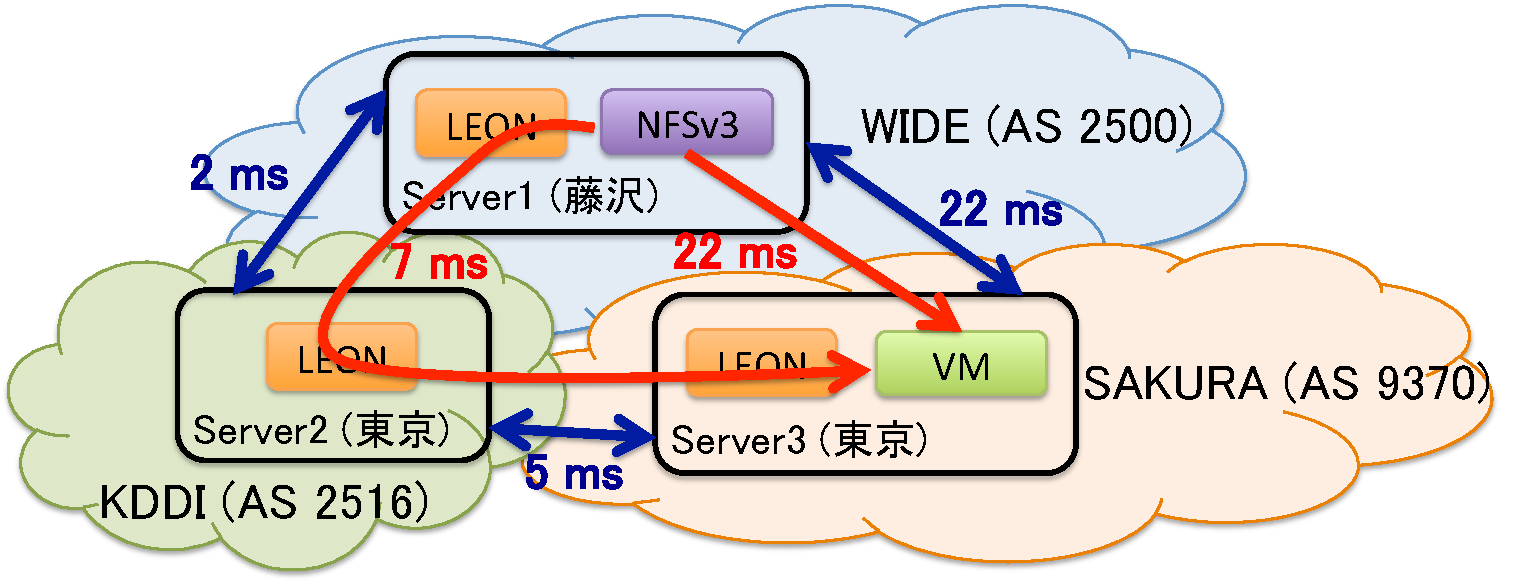
\includegraphics[scale=0.65]{./img/spexp}
		\caption{サービスパフォーマンス計測に用いた実験環境}
		\label{img:spexp}
	\end{center}
\end{figure}

実験環境に対する要求から、本実験を行うにあたり、インターネット上に分散された3つの拠点に設置された3台のサーバーを利用して実験環境を構築した。
この実験環境のトポロジー図を図~\ref{img:spexp}に示す。また、利用した実機サーバーの仕様を表~\ref{table:spserv}に示す。
更に、それぞれのサーバーで利用したソフトウェアのバージョンを表~\ref{table:spversion}に示す。Server 1はWIDE Projectの藤沢NOCに設置されたサーバーである。
Server 2はKDDIウェブコミュニケーションズ社~\cite{kddiwebcom}が提供しているCloudCore VPSサービス~\cite{cloudcore}を利用した
仮想サーバーである。そして、Server 3はEditNet社~\cite{editnet}による
フレッツ光ネクスト接続サービス~\cite{enflets}~\cite{nttflets}を用いて接続されたサーバーである。
EditNet社のサービスはさくらインターネット社~\cite{sakurainc}のバックボーンを利用している~\cite{enbb}。

実験を行うにあたり、これら3台のサーバーでLEONの実装であるleondを動作させた。WIDE Projectとさくらインターネットは堂島でピアリングを行なっている。
そのため、Server 1とServer 3が直接通信した場合、堂島を経由するために遅延が22 ms以上かかる。一方、WIDE ProjectとKDDIは東京でピアリングを行なっている。
また、KDDIとさくらインターネットも同様に、東京でピアリングを行なっている。そのため、Server 1とServer 3が通信を行うにはServer 2を経由することにより、
直接通信した場合よりも小さい遅延で通信をすることができる。leondはこの経路を自動的に発見し、Server 1からServer 3宛のイーサネットフレームを転送する際には
Server 2を経由させ転送をする。

\begin{table}[h]
\begin{center}
	\caption{サービスパフォーマンス計測に用いたサーバーの仕様}
	\begin{tabular}{|l|l|l|l|}
		\hline
		ホスト & CPU & メモリー & NIC \\
		\hline
		\hline
		Server 1 (藤沢) & Intel Xeon L5520 2.27GHz & 12GB & NetXtreme II BCM5709 \\
		\hline
		Server 2 (東京) & AMD Phenom 9550 2.20GHz& 2GB & virtio \\
		\hline
		Server 3 (東京) & Intel i7 870 2.93GHz & 16GB & Intel 82574L \\
		\hline
	\end{tabular}
	\label{table:spserv}
\end{center}
\end{table}

\begin{table}[h]
\begin{center}
	\caption{サービスパフォーマンス計測に用いた各サーバーのソフトウェアバージョン}
	\begin{tabular}{|l|l|l|l|}
		\hline
		サーバー & OS & Linux Kernel & gcc \\
		\hline
		\hline
		Server 1 (藤沢) & Debian GNU/Linux 6.0.6 Squeeze & 3.7.2 & 4.4.5 \\
		\hline
		Server 2 (東京) & Fedora 17			 & 3.7.4-204 & 4.7.2 \\
		\hline
		Server 3 (東京)	& Fedora 15			 & 2.6.43.8-1 & 4.6.3 \\
		\hline
	\end{tabular}
	\label{table:spversion}
\end{center}
\end{table}

これにより、3台のサーバーを用いて、本実験を行うための要求を満たした実験環境を構築した。

本評価を行うにあたり、NFSv3のファイルシステムパフォーマンスと仮想マシン内でのLinux Kernel
コンパイル所要時間を計測した。本実験は、NFSv3の通信を直接インターネット上で行った場合と、
LEONを利用して構築されたLayer 2ネットワーク上で行った場合の2通りで計測した。本実験を行うにあたり、
~\ref{spexpenv}節で説明した実験環境において、Server 1をストレージサーバー、Server 3を仮想マシンを
動かすサーバーとした。Server 1のディスク領域をNFSv3を利用してServer 3から利用できるようにした。

NFSv3のファイルシステムパフォーマンスの計測にはBonnie++~\cite{bonnieplusplus}を用いた。Bonnie++はRussel Coker氏に
よって開発されたディスク・ファイルシステムパフォーマンス計測ツールである。本実験では、Server 3上でBonnie++を動作させ、NFSv3の
シーケンシャルアクセスパフォーマンスとランダムアクセスパフォーマンスを計測した。

また、仮想マシン内でのLinux Kernelコンパイル所要時間を計測するために、Server 3上で仮想マシンを動作させた。
仮想マシンを動作させるための仮想化技術にはKernel-based Virtual Machine(=KVM)~\cite{kvm}を利用した。また、仮想マシンの
ディスクイメージはServer 1に記憶されており、NFSv3を経由して仮想マシンに提供される。仮想マシンの内部で
Linux Kernelのコンパイルを行い、Linux Kernelのコンパイルにかかる時間をtimeコマンドを用いて計測した。

サービスのパフォーマンス計測としてまず、NFSv3のファイルシステムパフォーマンスを計測した。計測はインターネット上の経路
で直接NFSv3の通信を行った場合とLEONを利用して拡張されたLayer 2ネットワーク上でNFSv3の通信を行った場合の2通りで計測を
行った。シーケンシャルアクセスパフォーマンスの計測結果を表~\ref{nfsseq}、ランダムアクセスパフォーマンスの計測結果を
表~\ref{nfsrand}に示す。計測はそれぞれ3回行い、計測結果は3回の平均値である。

\begin{table}[h]
        \begin{center}
                \caption{NFSv3のシーケンシャルアクセスパフォーマンス}
                \begin{tabular}{|l|l|l|}
                        \hline
                                通信手法 & read (K/sec) & write (K/sec) \\
                        \hline
			\hline
                                Direct & 4537 & 5372 \\
			\hline
				LEON & 4726 & 5198 \\
                        \hline
                \end{tabular}
                \label{nfsseq}
        \end{center}
\end{table}

\begin{table}[h]
        \begin{center}
                \caption{NFSv3のランダムアクセスパフォーマンス}
                \begin{tabular}{|l|l|l|l|l|}
                        \hline
                                通信手法 & seek(/sec) & create(/sec) & info(/sec) & delete(/sec) \\
                        \hline
			\hline
                                Direct & 2985 & 23 & 46 & 46 \\
			\hline
				LEON & 8417 & 65 & 132 & 132\\
                        \hline
                \end{tabular}
                \label{nfsrand}
        \end{center}
\end{table}

インターネット上の経路で直接通信を行った場合のシーケンシャルアクセスパフォーマンスは、読み込み速度が4537 K/sec、
書き込み速度が5372 K/secであった。一方、LEONを利用して拡張されたLayer 2ネットワーク上で通信を行った場合のシーケンシャル
アクセスパフォーマンスは、読み込み速度が4726 K/sec、書き込み速度が5198 K/secであった。この計測結果から、シーケンシャル
アクセスのパフォーマンスは、インターネット上の経路で直接通信を行った場合と、LEONを利用して拡張されたLayer 2ネットワーク上で
通信を行った場合では、大きは変化はないということがわかった。

一方、インターネット上の経路で直接通信を行った場合のランダムアクセスパフォーマンスは、seek操作が毎秒2985回、create操作
が毎秒23回、info操作が毎秒46回、delete操作が毎秒46回という結果となった。LEONを利用して拡張されたLayer 2ネットワーク上で通信を行った場合
では、seek操作が毎秒8417回、create操作が毎秒65回、info操作が毎秒132回、delete操作が毎秒132回であった。この計測結果から、
ランダムアクセスのパフォーマンスは、インターネット上の経路で直接通信を行った場合に比べ、LEONを利用して拡張されたLayer 2ネットワーク上で
通信を行った場合では約3倍のパフォーマンスとなることがわかった。

次に、サービスのパフォーマンス計測として、仮想マシン内でのLinux Kernelのコンパイル所要時間を計測した。その計測結果を表~\ref{kernelcompile}に示す。
インターネット上の経路で直接通信を行った場合のコンパイル所要時間は78.9分であった。一方、LEONを利用して拡張されたLayer 2ネットワーク上で通信を行った場合
のコンパイル所要時間は58.8分であった。LEONを利用して拡張されたLayer 2ネットワーク上で通信を行うことにより、直接通信を行った場合と比べ、コンパイル所要時間
を約20分削減できることがわかった。

\begin{table}[tb]
        \begin{center}
                \caption{Kernelコンパイルの所要時間}
                \begin{tabular}{|l|l|}
                        \hline
                                通信手法 & コンパイル所要時間 (分) \\
                        \hline
			\hline
                                Direct & 78.9 \\
			\hline
				LEON & 58.8\\
                        \hline
                \end{tabular}
                \label{kernelcompile}
        \end{center}
\end{table}

本研究では、LEONがサービスのパフォーマンスに与える影響を評価した。本評価を行うために、インターネット上の経路で
直接通信した場合と、LEONを利用して拡張されたLayer 2ネットワーク上で通信を行った場合のNFSv3のファイルシステムパフォーマンス
と仮想マシン内でのLinux Kernelコンパイル所要時間を計測した。

LEONを利用することによりランダムアクセスパフォーマンスは改善されたが、シーケンシャルアクセスパフォーマンスは改善されなかった。
NFSv3のシーケンシャルアクセスのパフォーマンスはサーバー間の帯域に依存すると考えられる。今回構築した実験環境では、
フレッツ光ネクスト接続サービスを用いてインターネットに接続されたサーバーの帯域が細いため、このサーバーの回線が
帯域のボトルネックとなっている。そのため、シーケンシャルアクセスのパフォーマンスは改善されなかったと考えられる。
一方、NFSv3のランダムアクセスのパフォーマンスはサーバー間の遅延に依存すると考えられる。NFSv3において1秒間に行える
ランダムアクセスの回数は、1秒間にサーバー間で何回NFSv3のパケットをやり取りできるかに比例する。LEONを利用することにより、
サーバー間の遅延は小さくなる。そのため、1秒間にサーバー間でやり取りできるパケット数が大きくなったため、ランダムアクセス
のパフォーマンスが改善されたと考えられる。

NFSv3のランダムアクセスのパフォーマンスが改善されることにより、仮想マシン内でのLinux Kernelコンパイル
所要時間は約20分短縮された。仮想マシン内でのLinux Kernelコンパイル作業では多くのランダムアクセスが生じると
予想される。そのため、NFSv3のランダムアクセスのパフォーマンスが改善されたため、仮想マシン内でより高速な
ランダムアクセスが可能になったため、Linux Kernelコンパイル所要時間が短縮されたと考えられる。

本実験の実験結果から、LEONを利用することにより、サービスのパフォーマンスは改善されるということがわかった。
LEONは遅延の最も小さい経路でイーサネットフレームの転送を行う。これにより、直接通信した場合と比べ、小さい遅延で
のLayer 2ネットワーク上のコンポーネント間の通信を可能とする。そのため、コンポーネントのパフォーマンスが改善され、
サービスのパフォーマンスが改善される。

\section{その他の実装}

本研究では次に、トンネル終端点の増加がLEONに与える影響の評価を行う。LEONを利用してLayer 2ネットワークを拡張している
トンネル終端点の台数が増加すると様々な影響が生じると考えられる。生じる影響の1つとして中継を行なっているトンネル終端点
において障害が発生してから、通信が復旧するまでの時間の増加が考えられる。本研究では、このような障害が発生してから通信復旧
までにかかる時間に着目した。

LEONは宛先のトンネル終端点に、遅延の最も小さい経路で、イーサネットフレームを転送する。これを行うため、LEONでは、
~\ref{solv:latencyprotocol}項で説明したような遅延データベースを構築する。そして、遅延データベースを用いて、
Layer 2ネットワークに参加している1つ1つのトンネル終端点までの遅延が最も小さくなる経路を事前に計算し、拡張された
Layer 2ネットワークのトポロジーを作成している。イーサネットフレームはこのトポロジーに基いて転送される。

VXLANとN2Nは遅延の最も小さい経路でイーサネットフレームの転送を行わないため、拡張されたLayer 2ネットワーク
のトポロジーを作成しない。トポロジーを作成しない利点として、Layer 2ネットワークに参加している何れかのトンネル終端点で障害が
発生しても、拡張されたLayer 2ネットワークにおいて障害は発生しないという点が挙げられる。VXLANの場合、何れかのトンネル終端点
で障害が発生しても、IPマルチキャストが正常に動作していればLayer 2ネットワーク上での通信は正常に行える。同様に、N2Nの場合でも、
Supernodeで障害が発生しなければLayer 2ネットワーク上での通信は正常に行える。そのため、トポロジーを作成しないVXLANとN2Nでは、
あるトンネル終端点で発生した障害によって拡張されたLayer 2ネットワークが影響を受けることはない。

一方で、遅延の最も小さい経路でイーサネットフレームの転送を行うためにトポロジーを作成するLEONは、ある終端点で発生した障害によって
拡張されたLayer 2ネットワークが一時的に影響を受ける場合がある。これは、障害が発生したトンネル終端点が、イーサネットフレームの
中継を行なっていた場合ある。中継を行なっているトンネル終端点で障害が発生すると、そのトンネル終端点を経由する経路が全て利用できなくなる。
LEONは遅延計測を行うと同時に、トンネル終端点の死活監視も行なっている。障害を検知すると、障害が発生しているトンネル終端点をトンネル終端点リスト
から削除し、経路の再計算を行う。しかし、LEONではデフォルトで遅延計測を60秒に1回で行なっていて、遅延計測メッセージの応答が2回ない場合に障害発生と判断している。
そのため、障害が発生から検知までに最大120秒を必要とする。検知してトポロジーが収束するまでは、障害が発生したトンネル終端点にイーサネットフレーム
を転送し続けるため、障害が発生したトンネル終端点を経由する通信は宛先に到達できなくなる。

また、LEONでは拡張されたLayer 2ネットワークに参加している全てのトンネル終端点が、それぞれ異なるトポロジーを作成している。
そのため、あるトンネル終端点で障害が発生してからLayer 2ネットワーク上の通信が完全に正常に戻るには、全てのトンネル終端点が障害を検知し、
トポロジーを作成し直す必要がある。つまり、障害が発生してから復旧までかかる時間は、Layer 2ネットワークに参加しているトンネル終端点の台数の影響を受ける可能性があると
考えられる。

そこで本評価では、Layer 2ネットワークに参加しているトンネル終端点の台数が、あるトンネル終端点の障害が発生してからLayer 2ネットワーク
の通信が正常化するまでかかる時間に与える影響を調査する。調査を行うために、トンネル終端点を徐々に増加させ、障害発生から全てのトンネル終端点で
のトポロジー収束までかかる時間を計測する。具体的には、全てのトンネル終端点の通信を中継しているトンネル終端点で障害を発生させ、そのトンネル終端点を
経由していた通信が復旧するまでにかかる時間を計測する。この計測をトンネル終端点の台数を変化させながら行う。

本研究では、イーサネットフレームの転送を中継しているトンネル終端点で障害が発生した際に、Layer 2ネットワークに参加
しているトンネル終端点の台数が、トポロジーの収束時間に与える影響を評価する。評価を行うにあたり、Layer 2ネットワーク
に参加しているトンネル終端点の台数を変化させ、それぞれの場合での障害発生から
全てのトンネル終端点でトポロジーが収束するまでにかかる時間を計測する。この計測を行うにあたって、実験環境に対して
以下の要求が受けられる。

\begin{itemize}
	\item{全てのトンネル終端点間に遅延が存在すること}
	\item{直接通信するよりも小さい遅延で通信することができる経路が存在すること}
	\item{数十台のトンネル終端点}
\end{itemize}

LEONはインターネット上に分散された複数の拠点に同一のLayer 2ネットワークを拡張する
ために利用される。インターネットにおいて、分散された複数の拠点同士が通信するにあたり、遅延が生じる。そのため、実験環境を
実インターネット環境と類似した環境にするためには、実験環境のトンネル終端点間に遅延が存在する必要がある。

また、本実験では、中継をするトンネル終端点で障害が発生してから、全てのトンネル終端点でトポロジーが収束するまでの時間を計測する。
この計測を行うには、あるトンネル終端点がイーサネットフレームを転送する際に、中継するトンネル終端点が必要となる。LEONは直接
宛先のトンネル終端点へ転送するよりも、他のトンネル終端点を経由して宛先のトンネル終端点へ転送することにより、小さい遅延で転送できるような
経路が存在した場合に中継するトンネル終端点を設定する。そのため、実験環境では、直接通信するよりも小さい遅延で通信することができる経路が必要となる。

さらに、~\ref{solv:env}節で説明したように、LEONは数十の拠点にLayer 2ネットワークを拡張することを想定している。
想定環境と類似した環境で実験を行うため、実験は最大で数十台のトンネル終端点という規模で行う。

\begin{figure}
	\begin{center}
		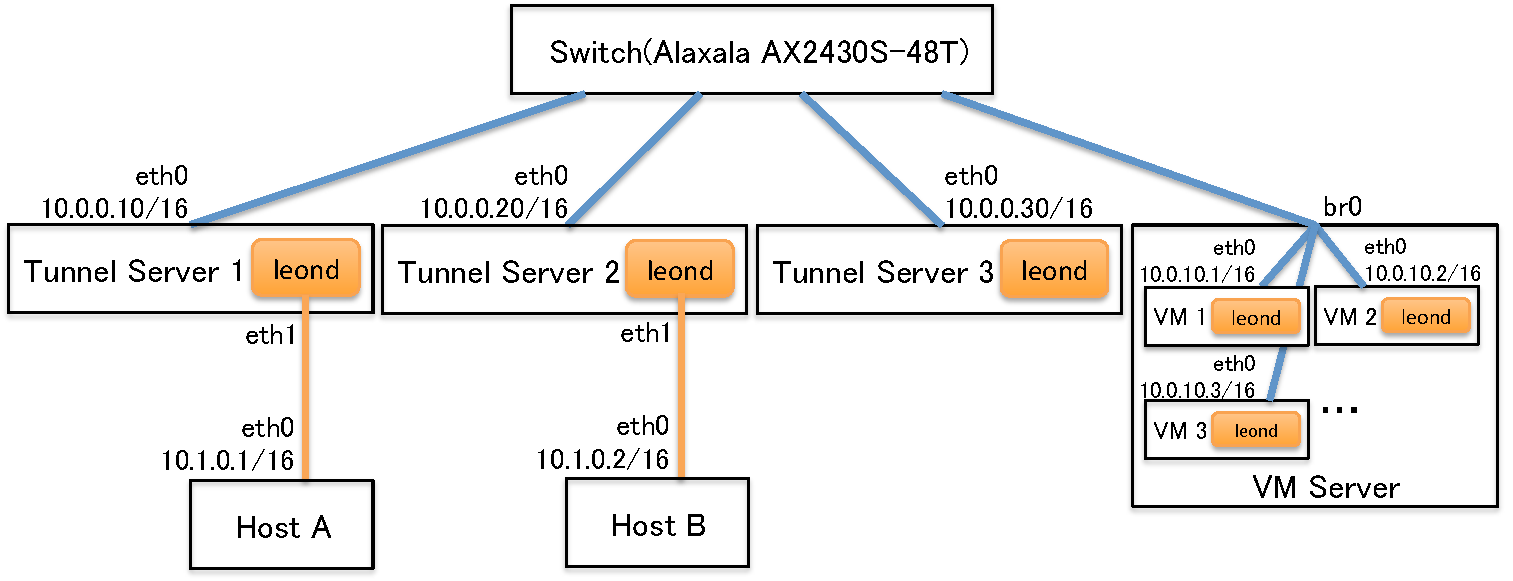
\includegraphics[scale=0.65]{./img/experimenttopology}
		\caption{実験環境のトポロジー図}
		\label{img:experimenttopology}
	\end{center}
\end{figure}

%%% Local Variables:
%%% mode: japanese-latex
%%% TeX-master: "../yummy_bthesis"
%%% End:
